\vzmstitle[
	\footnote{Работа поддержана грантом РНФ №17-11-01303}
]{
	Инварианты Фоменко-Цишанга невыпуклых топологических биллиардов
}

\vzmsauthor{Ведюшкина}{В.\,В.}

\vzmsinfo{Москва; {\it arinir@yandex.ru}}

\vzmscaption

Зададим семейство софокусных квадрик уравнением
$$(b-\lambda)x^2+(a-\lambda)y^2=(a-\lambda)(b-\lambda),   \lambda\leqslant a.    $$
Здесь $\infty> a> b>0$ --- фиксированная   пара чисел, $\lambda$ ---
параметр, определяющий квадрику.

Пусть  компактная область $\Omega$  на плоскости $\mathbb{R}^2$  такова,
что её граница  является объединением кусочно-гладких \!\!\;кривых,
состоящих из дуг софокусных квадрик, причём в точках излома  углы равны $\frac{\pi}{2}$. Такую область назовём элементарной.
Рассмотрим   биллиард  в ней, описываемый движением   точки внутри  $\Omega$ с
абсолютно упругим отражением на границе. В точках,
где граница   не гладкая
(тогда   угол излома  равен $\frac{\pi}{2}$)
 траектории системы  доопределим по непрерывности:  попав в вершину угла, материальная точка, не теряя скорости, отразится назад по той же траектории.  Будем называть такие биллиарды элементарными биллиардами.
 Такая система   интегрируема: помимо квадрата модуля вектора скорости   вдоль траекторий биллиарда сохраняется функция $\Lambda$ -- параметр софокусной квадрики: прямые, содержащие звенья ломаной-траектории биллиарда являются касательными к некоторой квадрике с фиксированным параметром $\Lambda$, принадлежащей тому же семейству квадрик что и граница биллиарда [2].

\textbf{Определение.}
{\it Невыпуклым  топологическим   биллиардом   назовём биллиард,  склеенный из конечного числа элементарных биллиардов вдоль общих   сегментов границ, которые могут быть как выпуклыми так и невыпуклыми.}

Материальная точка  топологического биллиарда дви\-же\-т\-ся внутри каждой из областей вдоль отрезков прямых,
переходя из одной области в другую при попадании на границу склейки.
Ранее автором была получена ли\-у\-вил\-ле\-ва классификация всех  топологических биллиардов,
полученных склейками вдоль выпуклых границ [3].

\textbf{Теорема.}
{\it Инварианты Фоменко--Цишанга~--- меченые молекулы $W^*$,
описывающие топологию слоения Лиувилля изоэнергетической поверхности $Q^3$
ограниченных дугами софокусных квадрик интегрируемых топологических биллиардов (как выпуклых, так и невыпуклых),
внутренность которых имеет пустое пересечение с фокальной прямой,   изображены на рисунке \ref{moleculesSimple}.
}
 \begin{figure}[h!]

   \center{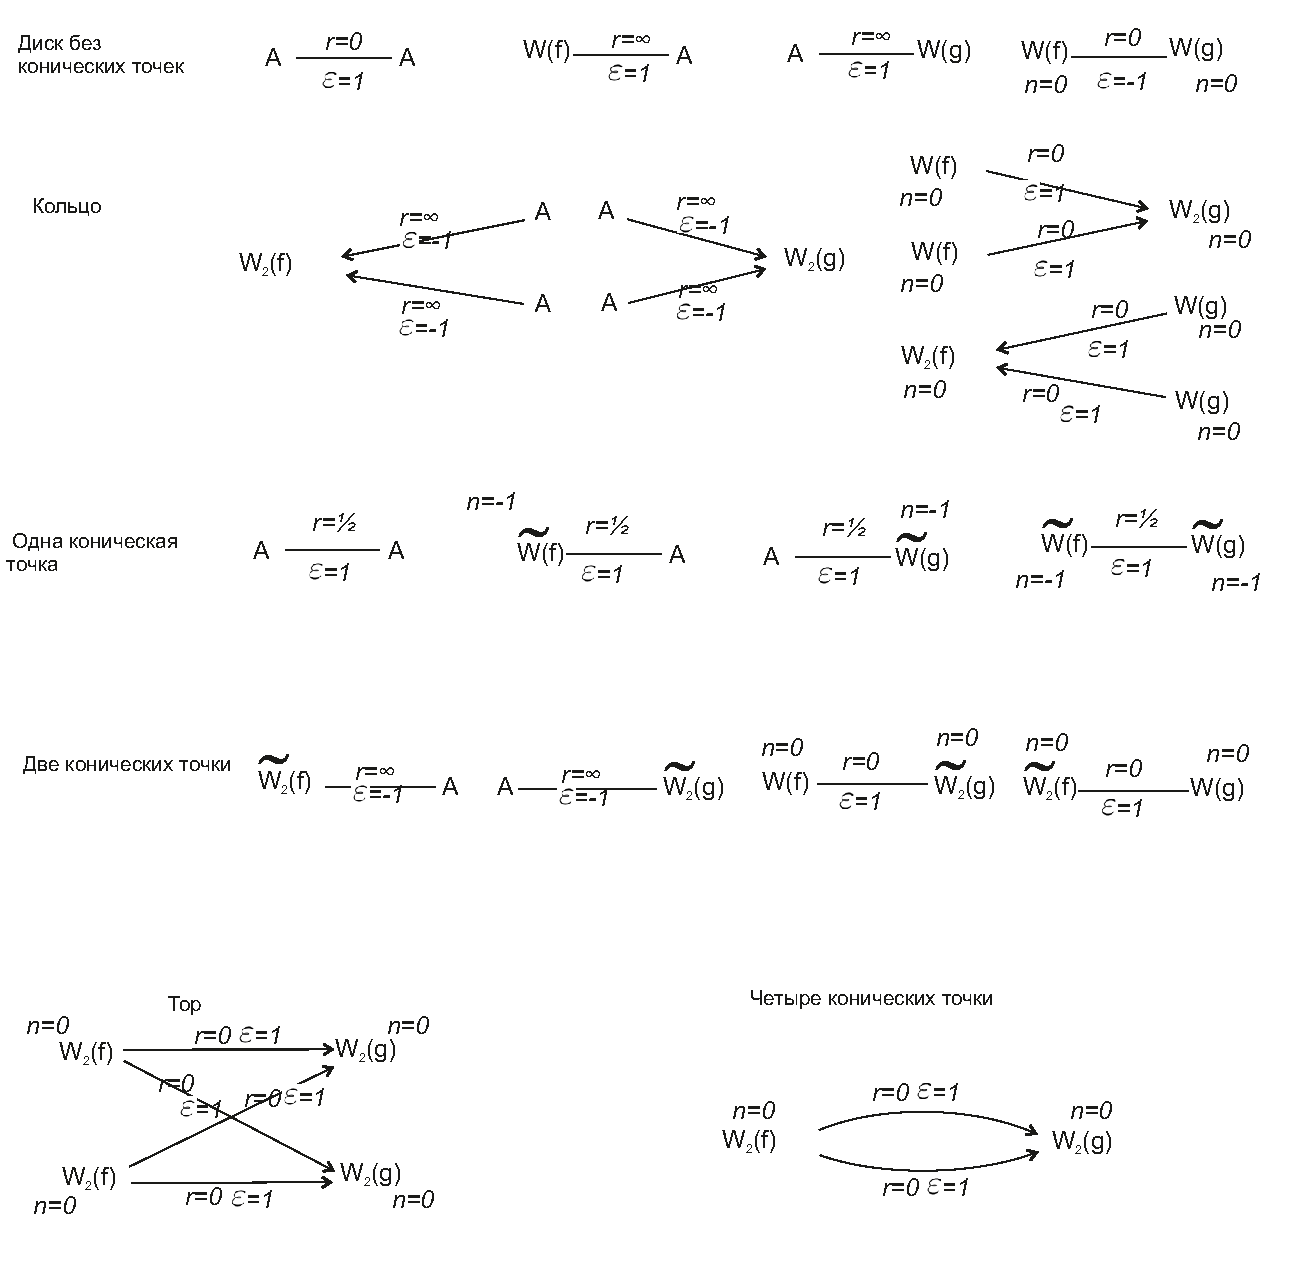
\includegraphics[width=100mm]{Vedushkina_moleculesSimple.pdf}}
\caption{Инварианты Фоменко-Цишанга топологических    биллиардов, внутренность которых имеет пустое пересечение с фокальной прямой}
\label{moleculesSimple}
 \end{figure}


 В докладе будет представлена полная классификация биллиардных областей и полная классификация их инвариантов Фоменко-Цишанга.



\litlist

1. {\it Болсинов А.\,В, Фоменко А.\,Т.} Интегрируемые гамильтоновы системы.
Геометрия, топология, классификация,
\linebreak
Т.1,2,
   Ижевск
   НИЦ ``Регулярная и хаотическая динамика'',
  1999

2. {\it  Фоменко А.Т., Цишанг Х.} О типичных топологических свойствах
интегрируемых гамильтоновых систем,  Изв. АН СССР
   52:2(1988),
  378--407


  3. {\it Козлов В.В., Трещёв Д.В.} Генетическое  введение в динамику систем с ударами. М.: Изд-во МГУ, 1991

4.  {\it Ведюшкина В.В.} Топологическая классификация биллиардов в локально плоских областях,
ограниченных дугами софокусных квадрик, Матем. сб., 206:10 (2015), 127-176

  5. {\it Ведюшкина В.В.} Слоение Лиувилля невыпуклых топологических биллиардов, ДАН, 478:1(2018)

